\chapter{Derivadas y aplicaciones}

\begin{theorybox}{Trazabilidad del capitulo}
Este capitulo desarrolla las secciones \texttt{C09.S01-C09.S08} de la matriz de cobertura a
partir de \texttt{sources/Relacion ejercicios tema 9. Derivadas y sus aplicaciones.pdf}. Se
separan con claridad los apartados nucleares de reglas, estudio local y global, rectas
tangentes, parametros, derivabilidad y optimizacion, dejando el bloque de ampliacion marcado
como \texttt{C09.S08}.
\end{theorybox}

\section{[C09.S01] Reglas de derivacion}

\subsection*{Objetivos de aprendizaje}
\begin{itemize}
  \item Aplicar con seguridad las reglas basicas de derivacion.
  \item Distinguir cuando conviene usar suma, producto, cociente o cadena.
  \item Simplificar el resultado sin perder la estructura de la derivada.
\end{itemize}

\subsection*{Prerrequisitos}
\begin{itemize}
  \item Operaciones con polinomios, radicales, logaritmos y exponenciales.
  \item Reconocer una composicion de funciones sencilla.
\end{itemize}

\begin{theorybox}{Reglas minimas de trabajo}
Si \(f\) y \(g\) son derivables, entonces:
\[
(f+g)'=f'+g',\qquad (kf)'=kf',\qquad (fg)'=f'g+fg',
\]
\[
\left(\frac{f}{g}\right)'=\frac{f'g-fg'}{g^2}\quad (g\neq 0),
\qquad (f\circ g)'=(f'\circ g)\cdot g'.
\]
Ademas,
\[
(x^n)'=nx^{n-1},\qquad (\sen x)'=\cos x,\qquad (\cos x)'=-\sen x,
\]
\[
(e^x)'=e^x,\qquad (\ln x)'=\frac{1}{x}.
\]
\end{theorybox}

\begin{methodbox}{Como reconocer la regla adecuada}
\begin{enumerate}
  \item Separa primero las sumas o restas exteriores.
  \item Si ves dos factores multiplicandose, prueba la regla del producto.
  \item Si aparece una fraccion, piensa en el cociente.
  \item Si una funcion esta ``metida dentro'' de otra, activa la regla de la cadena.
  \item Solo al final simplifica; antes conviene conservar la estructura para no perder signos.
\end{enumerate}
\end{methodbox}

\begin{solvedexample}{[EX-C09.S01-01] Producto con radical}
Deriva
\[
f(x)=(x^2+1)\sqrt{x+2}.
\]

\textbf{Lectura del enunciado.} Hay un producto entre un polinomio y una raiz, asi que la
estructura dominante es la regla del producto. Dentro de la raiz aparece ademas una funcion
lineal, por lo que se usa tambien la cadena.

\textbf{Desarrollo.} Si
\[
u(x)=x^2+1,\qquad v(x)=\sqrt{x+2}=(x+2)^{1/2},
\]
entonces
\[
u'(x)=2x,\qquad v'(x)=\frac{1}{2}(x+2)^{-1/2}\cdot 1=\frac{1}{2\sqrt{x+2}}.
\]
Por tanto,
\[
f'(x)=u'v+uv'=2x\sqrt{x+2}+\frac{x^2+1}{2\sqrt{x+2}}.
\]

\textbf{Comprobacion.} El primer sumando viene de derivar el polinomio y el segundo de derivar
la raiz. No falta ningun factor de cadena.

\textbf{Respuesta final.}
\[
f'(x)=2x\sqrt{x+2}+\frac{x^2+1}{2\sqrt{x+2}}.
\]
\end{solvedexample}

\begin{commonerror}{Derivar la raiz como si fuera \(\sqrt{x}\)}
En \(\sqrt{x+2}\) no basta escribir \(\frac{1}{2\sqrt{x+2}}\) por intuicion y olvidarse del
interior. En este ejemplo el interior deriva a \(1\), pero en \(\sqrt{2x+5}\) apareceria un
factor adicional \(2\). Conviene escribir la cadena de forma explicita antes de simplificar.
\end{commonerror}

\begin{guidedexercise}{[GX-C09.S01-01] Cociente}
Deriva
\[
g(x)=\frac{3x^2-1}{x+1}.
\]
\end{guidedexercise}

\begin{shortanswer}{[GX-C09.S01-01]}
\[
g'(x)=\frac{3x^2+6x+1}{(x+1)^2}.
\]
\end{shortanswer}

\begin{fullsolution}{[GX-C09.S01-01]}
Aplicamos el cociente:
\[
g'(x)=\frac{(6x)(x+1)-(3x^2-1)\cdot 1}{(x+1)^2}
=\frac{6x^2+6x-3x^2+1}{(x+1)^2}
=\frac{3x^2+6x+1}{(x+1)^2}.
\]
\end{fullsolution}

\begin{guidedexercise}{[GX-C09.S01-02] Cadena con radical}
Deriva
\[
h(x)=\sqrt{2x+5}.
\]
\end{guidedexercise}

\begin{shortanswer}{[GX-C09.S01-02]}
\[
h'(x)=\frac{1}{\sqrt{2x+5}}.
\]
\end{shortanswer}

\begin{fullsolution}{[GX-C09.S01-02]}
Escribimos \(h(x)=(2x+5)^{1/2}\). Entonces
\[
h'(x)=\frac{1}{2}(2x+5)^{-1/2}\cdot 2=\frac{1}{\sqrt{2x+5}}.
\]
\end{fullsolution}

\subsection*{Practica autonoma graduada}
\begin{exercise}{[PX-C09.S01-01] Deriva \(f(x)=x^4-3x+2\).}
\end{exercise}
\begin{exercise}{[PX-C09.S01-02] Deriva \(f(x)=(x^2+1)(x-3)\).}
\end{exercise}
\begin{exercise}{[PX-C09.S01-03] Deriva \(f(x)=\dfrac{2x+1}{x-2}\).}
\end{exercise}
\begin{exercise}{[PX-C09.S01-04] Deriva \(f(x)=\sqrt{x^2+4}\).}
\end{exercise}
\begin{exercise}{[PX-C09.S01-05] Deriva \(f(x)=e^{3x}\).}
\end{exercise}
\begin{exercise}{[PX-C09.S01-06] Deriva \(f(x)=\ln(x^2+1)\).}
\end{exercise}
\begin{exercise}{[PX-C09.S01-07] Deriva \(f(x)=\sen x\cos x\).}
\end{exercise}
\begin{exercise}{[PX-C09.S01-08] Deriva \(f(x)=(x^2-1)^3\).}
\end{exercise}

\begin{shortanswer}{C09.S01 practica autonoma}
\begin{enumerate}[label=\textbf{PX-C09.S01-\arabic*:}, leftmargin=*]
  \item \(4x^3-3\)
  \item \(3x^2-6x+1\)
  \item \(-\dfrac{5}{(x-2)^2}\)
  \item \(\dfrac{x}{\sqrt{x^2+4}}\)
  \item \(3e^{3x}\)
  \item \(\dfrac{2x}{x^2+1}\)
  \item \(\cos^2 x-\sen^2 x\)
  \item \(6x(x^2-1)^2\)
\end{enumerate}
\end{shortanswer}

\begin{fullsolution}{C09.S01 practica autonoma}
\begin{enumerate}[label=\textbf{PX-C09.S01-\arabic*:}, leftmargin=*]
  \item \((x^4-3x+2)'=4x^3-3\).
  \item
  \[
  f'(x)=2x(x-3)+(x^2+1)=3x^2-6x+1.
  \]
  \item
  \[
  f'(x)=\frac{2(x-2)-(2x+1)}{(x-2)^2}=-\frac{5}{(x-2)^2}.
  \]
  \item
  \[
  f'(x)=\frac{1}{2}(x^2+4)^{-1/2}\cdot 2x=\frac{x}{\sqrt{x^2+4}}.
  \]
  \item \((e^{3x})'=3e^{3x}\).
  \item
  \[
  (\ln(x^2+1))'=\frac{2x}{x^2+1}.
  \]
  \item
  \[
  (\sen x\cos x)'=\cos x\cos x+\sen x(-\sen x)=\cos^2 x-\sen^2 x.
  \]
  \item
  \[
  \bigl((x^2-1)^3\bigr)'=3(x^2-1)^2\cdot 2x=6x(x^2-1)^2.
  \]
\end{enumerate}
\end{fullsolution}

\section{[C09.S02] Monotonia, extremos, curvatura e inflexion}

\subsection*{Objetivos de aprendizaje}
\begin{itemize}
  \item Usar la primera derivada para localizar crecimiento y decrecimiento.
  \item Clasificar maximos y minimos locales con el cambio de signo de \(f'\).
  \item Leer la concavidad y los puntos de inflexion con la segunda derivada.
\end{itemize}

\subsection*{Prerrequisitos}
\begin{itemize}
  \item Calculo correcto de derivadas.
  \item Tablas de signos e interpretacion de intervalos.
\end{itemize}

\begin{theorybox}{Que nos dicen las derivadas}
Si \(f'(x)>0\), la funcion crece; si \(f'(x)<0\), decrece. Los puntos donde \(f'(x)=0\) o no
existe son candidatos a extremo. Para la curvatura:
\[
f''(x)>0 \Longrightarrow \text{concavidad hacia arriba},\qquad
f''(x)<0 \Longrightarrow \text{concavidad hacia abajo}.
\]
Un punto de inflexion aparece cuando cambia el signo de \(f''\).
\end{theorybox}

\begin{methodbox}{Esquema de estudio}
\begin{enumerate}
  \item Deriva una vez y resuelve \(f'(x)=0\).
  \item Ordena los puntos criticos y estudia el signo de \(f'\) entre ellos.
  \item Deriva una segunda vez si se pide curvatura o inflexion.
  \item Resume siempre con intervalos y con coordenadas de los puntos destacados.
\end{enumerate}
\end{methodbox}

\begin{solvedexample}{[EX-C09.S02-01] Cubica con maximo, minimo e inflexion}
Estudia monotonia, extremos y curvatura de
\[
f(x)=x^3-3x.
\]

\textbf{Desarrollo.} Derivamos:
\[
f'(x)=3x^2-3=3(x-1)(x+1).
\]
Los puntos criticos son \(x=-1\) y \(x=1\). El signo de \(f'\) queda:
\[
\begin{array}{c|ccc}
x & (-\infty,-1) & (-1,1) & (1,\infty)\\ \hline
f'(x) & + & - & +
\end{array}
\]
Por tanto, la funcion crece en \((-\infty,-1)\cup(1,\infty)\) y decrece en \((-1,1)\).

Calculamos los valores:
\[
f(-1)=2,\qquad f(1)=-2.
\]
Luego hay un maximo local en \((-1,2)\) y un minimo local en \((1,-2)\).

Ahora la segunda derivada:
\[
f''(x)=6x.
\]
Es negativa si \(x<0\) y positiva si \(x>0\), asi que la curvatura cambia en \(x=0\). Como
\[
f(0)=0,
\]
el punto de inflexion es \((0,0)\).

\textbf{Respuesta final.}
\begin{itemize}
  \item Crece en \((-\infty,-1)\cup(1,\infty)\).
  \item Decrece en \((-1,1)\).
  \item Maximo local en \((-1,2)\) y minimo local en \((1,-2)\).
  \item Concava hacia abajo en \((-\infty,0)\) y hacia arriba en \((0,\infty)\).
  \item Punto de inflexion en \((0,0)\).
\end{itemize}
\end{solvedexample}

\begin{commonerror}{Pensar que \(f'(a)=0\) implica automaticamente extremo}
Un punto con derivada nula solo es candidato. En \(f(x)=x^3\), por ejemplo, \(f'(0)=0\) y sin
embargo no hay maximo ni minimo. Siempre hay que mirar el signo de \(f'\) a ambos lados.
\end{commonerror}

\begin{guidedexercise}{[GX-C09.S02-01] Parabola}
Estudia la monotonia y el extremo de
\[
g(x)=x^2-4x+1.
\]
\end{guidedexercise}

\begin{shortanswer}{[GX-C09.S02-01]}
Decrece en \((-\infty,2)\), crece en \((2,\infty)\) y tiene minimo en \((2,-3)\).
\end{shortanswer}

\begin{fullsolution}{[GX-C09.S02-01]}
\[
g'(x)=2x-4=2(x-2).
\]
La derivada es negativa si \(x<2\) y positiva si \(x>2\). Por eso \(g\) decrece primero y
crece despues. Ademas,
\[
g(2)=4-8+1=-3,
\]
de modo que el minimo local es \((2,-3)\).
\end{fullsolution}

\begin{guidedexercise}{[GX-C09.S02-02] Inflexion sin extremo}
Estudia monotonia y curvatura de
\[
h(x)=x^3.
\]
\end{guidedexercise}

\begin{shortanswer}{[GX-C09.S02-02]}
Crece en todo \(\mathbb{R}\), es concava hacia abajo en \((-\infty,0)\), hacia arriba en
\((0,\infty)\) y tiene punto de inflexion en \((0,0)\).
\end{shortanswer}

\begin{fullsolution}{[GX-C09.S02-02]}
\[
h'(x)=3x^2\geq 0
\]
para todo \(x\), asi que la funcion es creciente en todo \(\mathbb{R}\). Ademas,
\[
h''(x)=6x,
\]
negativa si \(x<0\) y positiva si \(x>0\). Luego la concavidad cambia en \(x=0\) y el punto
de inflexion es \((0,0)\).
\end{fullsolution}

\subsection*{Practica autonoma graduada}
\begin{exercise}{[PX-C09.S02-01] Estudia monotonia y extremos de \(f(x)=-x^2+4x\).}
\end{exercise}
\begin{exercise}{[PX-C09.S02-02] Estudia monotonia, extremos e inflexion de \(f(x)=x^3-6x^2\).}
\end{exercise}
\begin{exercise}{[PX-C09.S02-03] Estudia monotonia y extremos de \(f(x)=x^4-2x^2\).}
\end{exercise}
\begin{exercise}{[PX-C09.S02-04] Halla los extremos absolutos de \(f(x)=x^2-4x+5\) en \([0,3]\).}
\end{exercise}
\begin{exercise}{[PX-C09.S02-05] Estudia monotonia y curvatura de \(f(x)=\ln x\).}
\end{exercise}
\begin{exercise}{[PX-C09.S02-06] Estudia monotonia y extremos de \(f(x)=e^x-x\).}
\end{exercise}

\begin{shortanswer}{C09.S02 practica autonoma}
\begin{enumerate}[label=\textbf{PX-C09.S02-\arabic*:}, leftmargin=*]
  \item Crece en \((-\infty,2)\), decrece en \((2,\infty)\) y tiene maximo en \((2,4)\)
  \item Crece en \((-\infty,0)\cup(4,\infty)\), decrece en \((0,4)\), maximo en \((0,0)\),
  minimo en \((4,-32)\) e inflexion en \((2,-16)\)
  \item Decrece en \((-\infty,-1)\cup(0,1)\), crece en \((-1,0)\cup(1,\infty)\), maximo en
  \((0,0)\) y minimos en \((-1,-1)\) y \((1,-1)\)
  \item Maximo absoluto \(5\) en \(x=0\); minimo absoluto \(1\) en \(x=2\)
  \item Crece en \((0,\infty)\), es concava hacia abajo en \((0,\infty)\) y no tiene inflexion
  \item Decrece en \((-\infty,0)\), crece en \((0,\infty)\) y tiene minimo en \((0,1)\)
\end{enumerate}
\end{shortanswer}

\begin{fullsolution}{C09.S02 practica autonoma}
\begin{enumerate}[label=\textbf{PX-C09.S02-\arabic*:}, leftmargin=*]
  \item
  \[
  f'(x)=-2x+4=-2(x-2).
  \]
  Es positiva si \(x<2\) y negativa si \(x>2\). Luego hay maximo en
  \[
  f(2)=4.
  \]
  \item
  \[
  f'(x)=3x^2-12x=3x(x-4),\qquad f''(x)=6x-12.
  \]
  De aqui salen los intervalos de crecimiento y decrecimiento, el maximo en \(x=0\), el
  minimo en \(x=4\) y el cambio de concavidad en \(x=2\). Los valores son
  \[
  f(0)=0,\qquad f(4)=-32,\qquad f(2)=-16.
  \]
  \item
  \[
  f'(x)=4x^3-4x=4x(x-1)(x+1).
  \]
  La tabla de signos produce los cuatro intervalos indicados. Los valores criticos son
  \[
  f(-1)=-1,\qquad f(0)=0,\qquad f(1)=-1.
  \]
  \item En \([0,3]\) comparamos extremos y punto critico interior:
  \[
  f(0)=5,\qquad f(2)=1,\qquad f(3)=2.
  \]
  \item
  \[
  f'(x)=\frac{1}{x}>0,\qquad f''(x)=-\frac{1}{x^2}<0
  \]
  para todo \(x>0\).
  \item
  \[
  f'(x)=e^x-1.
  \]
  Se anula en \(x=0\), es negativa si \(x<0\) y positiva si \(x>0\). Ademas,
  \[
  f(0)=1.
  \]
\end{enumerate}
\end{fullsolution}

\section{[C09.S03] Recta tangente y recta normal en un punto}

\subsection*{Objetivos de aprendizaje}
\begin{itemize}
  \item Interpretar la derivada en un punto como pendiente de la tangente.
  \item Escribir la ecuacion de la tangente y de la normal usando un punto de la curva.
  \item Reconocer el caso especial de tangente horizontal y normal vertical.
\end{itemize}

\subsection*{Prerrequisitos}
\begin{itemize}
  \item Reglas basicas de derivacion.
  \item Ecuacion de la recta en forma punto-pendiente.
\end{itemize}

\begin{theorybox}{Idea clave}
Si \(f\) es derivable en \(x=a\), la recta tangente en \(P(a,f(a))\) tiene pendiente
\(f'(a)\):
\[
y-f(a)=f'(a)(x-a).
\]
Si \(f'(a)\neq 0\), la recta normal tiene pendiente \(-1/f'(a)\). Si \(f'(a)=0\), la normal
es la recta vertical \(x=a\).
\end{theorybox}

\begin{methodbox}{Pasos fijos}
\begin{enumerate}
  \item Calcula el punto \(P(a,f(a))\).
  \item Deriva y halla la pendiente \(m_t=f'(a)\).
  \item Escribe la tangente con la forma punto-pendiente.
  \item Para la normal, usa la opuesta reciproca o escribe \(x=a\) si la tangente es
  horizontal.
\end{enumerate}
\end{methodbox}

\begin{center}
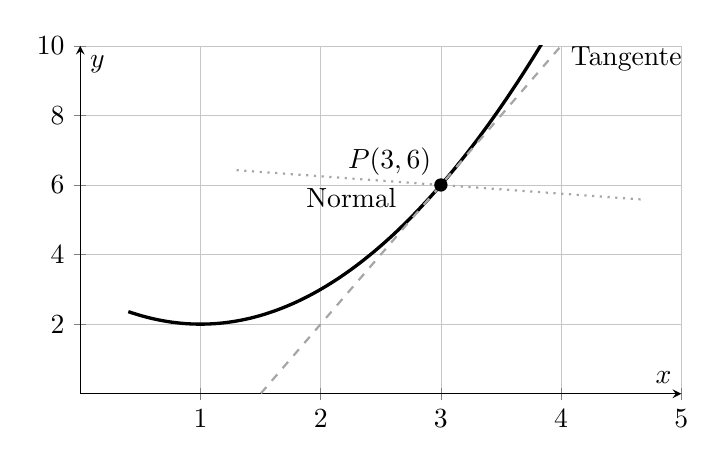
\begin{tikzpicture}
\begin{axis}[
  width=0.76\textwidth,
  height=6cm,
  axis lines=middle,
  xmin=0,
  xmax=5,
  ymin=0,
  ymax=10,
  samples=150,
  xlabel={$x$},
  ylabel={$y$},
  grid=both,
  grid style={line width=0.1pt, draw=gray!25},
  major grid style={line width=0.2pt, draw=gray!45},
]
\addplot[very thick, black, domain=0.4:4.6] {x^2 - 2*x + 3};
\addplot[thick, dashed, gray!70, domain=0.6:4.4] {4*x - 6};
\addplot[thick, dotted, gray!70, domain=1.3:4.7] {-x/4 + 27/4};
\addplot[only marks, mark=*, mark size=2.2pt] coordinates {(3,6)};
\node[anchor=south east] at (axis cs:3,6) {$P(3,6)$};
\node[anchor=south west] at (axis cs:4.0,9.0) {Tangente};
\node[anchor=north west] at (axis cs:1.8,6.2) {Normal};
\end{axis}
\end{tikzpicture}
\end{center}

\begin{solvedexample}{[EX-C09.S03-01] Tangente y normal a una parabola}
Calcula las ecuaciones de la tangente y la normal a
\[
f(x)=x^2-2x+3
\]
en \(x=3\).

\textbf{Desarrollo.} El punto de la curva es
\[
f(3)=9-6+3=6,
\]
luego \(P(3,6)\).

Derivamos:
\[
f'(x)=2x-2,\qquad f'(3)=4.
\]
La tangente es
\[
y-6=4(x-3)\Longrightarrow y=4x-6.
\]
La normal tiene pendiente \(-1/4\), asi que
\[
y-6=-\frac{1}{4}(x-3)\Longrightarrow y=-\frac{1}{4}x+\frac{27}{4}.
\]

\textbf{Respuesta final.}
\[
\text{Tangente: } y=4x-6,\qquad
\text{Normal: } y=-\frac{1}{4}x+\frac{27}{4}.
\]
\end{solvedexample}

\begin{commonerror}{Confundir normal con cambiar el signo}
La pendiente de la normal no es \(-m_t\), sino \(-1/m_t\). Solo cambiar el signo produce una
recta simetrica, no necesariamente perpendicular.
\end{commonerror}

\begin{guidedexercise}{[GX-C09.S03-01] Punto con pendiente negativa}
Calcula la tangente y la normal a
\[
f(x)=x^2+1
\]
en \(x=-1\).
\end{guidedexercise}

\begin{shortanswer}{[GX-C09.S03-01]}
Tangente: \(y=-2x\). Normal: \(y=\dfrac{x}{2}+\dfrac{5}{2}\).
\end{shortanswer}

\begin{fullsolution}{[GX-C09.S03-01]}
\[
f(-1)=2,\qquad f'(x)=2x,\qquad f'(-1)=-2.
\]
La tangente es
\[
y-2=-2(x+1)\Longrightarrow y=-2x.
\]
La normal tiene pendiente \(1/2\):
\[
y-2=\frac{1}{2}(x+1)\Longrightarrow y=\frac{x}{2}+\frac{5}{2}.
\]
\end{fullsolution}

\begin{guidedexercise}{[GX-C09.S03-02] Tangente horizontal}
Calcula la tangente y la normal a
\[
f(x)=x^3-3x
\]
en \(x=1\).
\end{guidedexercise}

\begin{shortanswer}{[GX-C09.S03-02]}
Tangente: \(y=-2\). Normal: \(x=1\).
\end{shortanswer}

\begin{fullsolution}{[GX-C09.S03-02]}
\[
f(1)=1-3=-2,\qquad f'(x)=3x^2-3,\qquad f'(1)=0.
\]
Por tanto la tangente es horizontal:
\[
y=-2.
\]
La normal es vertical, luego
\[
x=1.
\]
\end{fullsolution}

\subsection*{Practica autonoma graduada}
\begin{exercise}{[PX-C09.S03-01] Calcula la tangente y la normal a \(f(x)=x^2+2x\) en \(x=2\).}
\end{exercise}
\begin{exercise}{[PX-C09.S03-02] Calcula la tangente y la normal a \(f(x)=\dfrac{x+1}{x-1}\) en \(x=3\).}
\end{exercise}
\begin{exercise}{[PX-C09.S03-03] Calcula la tangente y la normal a \(f(x)=\sqrt{x+1}\) en \(x=3\).}
\end{exercise}
\begin{exercise}{[PX-C09.S03-04] Calcula la tangente y la normal a \(f(x)=e^x\) en \(x=0\).}
\end{exercise}
\begin{exercise}{[PX-C09.S03-05] Calcula la tangente y la normal a \(f(x)=\ln x\) en \(x=1\).}
\end{exercise}
\begin{exercise}{[PX-C09.S03-06] Calcula la tangente y la normal a \(f(x)=x^3\) en \(x=0\).}
\end{exercise}

\begin{shortanswer}{C09.S03 practica autonoma}
\begin{enumerate}[label=\textbf{PX-C09.S03-\arabic*:}, leftmargin=*]
  \item Tangente: \(y=6x-4\). Normal: \(y=-\dfrac{x}{6}+\dfrac{25}{3}\)
  \item Tangente: \(y=-\dfrac{x}{2}+\dfrac{7}{2}\). Normal: \(y=2x-4\)
  \item Tangente: \(y=\dfrac{x}{4}+\dfrac{5}{4}\). Normal: \(y=-4x+14\)
  \item Tangente: \(y=x+1\). Normal: \(y=-x+1\)
  \item Tangente: \(y=x-1\). Normal: \(y=-x+1\)
  \item Tangente: \(y=0\). Normal: \(x=0\)
\end{enumerate}
\end{shortanswer}

\begin{fullsolution}{C09.S03 practica autonoma}
\begin{enumerate}[label=\textbf{PX-C09.S03-\arabic*:}, leftmargin=*]
  \item
  \[
  f(2)=8,\qquad f'(x)=2x+2,\qquad f'(2)=6.
  \]
  Tangente:
  \[
  y-8=6(x-2)\Longrightarrow y=6x-4.
  \]
  Normal:
  \[
  y-8=-\frac{1}{6}(x-2)\Longrightarrow y=-\frac{x}{6}+\frac{25}{3}.
  \]
  \item
  \[
  f(3)=2,\qquad f'(x)=\frac{(x-1)-(x+1)}{(x-1)^2}=-\frac{2}{(x-1)^2},
  \]
  luego \(f'(3)=-1/2\). La tangente es
  \[
  y-2=-\frac{1}{2}(x-3)\Longrightarrow y=-\frac{x}{2}+\frac{7}{2}.
  \]
  La normal tiene pendiente \(2\):
  \[
  y-2=2(x-3)\Longrightarrow y=2x-4.
  \]
  \item
  \[
  f(3)=2,\qquad f'(x)=\frac{1}{2\sqrt{x+1}},\qquad f'(3)=\frac{1}{4}.
  \]
  \[
  y-2=\frac{1}{4}(x-3)\Longrightarrow y=\frac{x}{4}+\frac{5}{4}.
  \]
  La normal tiene pendiente \(-4\):
  \[
  y-2=-4(x-3)\Longrightarrow y=-4x+14.
  \]
  \item Como \(f(0)=1\) y \(f'(0)=1\),
  \[
  y-1=x\Longrightarrow y=x+1.
  \]
  La normal es
  \[
  y-1=-x\Longrightarrow y=-x+1.
  \]
  \item Como \(f(1)=0\) y \(f'(1)=1\),
  \[
  y=x-1,\qquad y=-x+1.
  \]
  \item
  \[
  f(0)=0,\qquad f'(0)=0.
  \]
  La tangente es \(y=0\) y la normal \(x=0\).
\end{enumerate}
\end{fullsolution}

\section{[C09.S04] Tangente con pendiente dada o paralela a una recta}

\subsection*{Objetivos de aprendizaje}
\begin{itemize}
  \item Traducir ``pendiente dada'' a una ecuacion con la derivada.
  \item Detectar si hay una, varias o ninguna tangente que cumpla la condicion.
  \item Escribir la recta final una vez localizada la abscisa de tangencia.
\end{itemize}

\subsection*{Prerrequisitos}
\begin{itemize}
  \item Derivacion y ecuacion de la recta tangente.
  \item Interpretacion geometrica de paralelismo entre rectas.
\end{itemize}

\begin{theorybox}{Traduccion directa}
Si se pide una tangente con pendiente \(m\), hay que resolver
\[
f'(x)=m.
\]
Cada solucion \(x=a\) genera un punto \(P(a,f(a))\) y, por tanto, una tangente:
\[
y-f(a)=m(x-a).
\]
\end{theorybox}

\begin{methodbox}{Ruta de resolucion}
\begin{enumerate}
  \item Deriva la funcion.
  \item Igualala a la pendiente pedida o a la pendiente de la recta dada.
  \item Resuelve la ecuacion para \(x\).
  \item Sustituye cada abscisa en la funcion y escribe las tangentes.
\end{enumerate}
\end{methodbox}

\begin{solvedexample}{[EX-C09.S04-01] Dos tangentes paralelas a la misma recta}
Halla las tangentes a
\[
f(x)=x^3-3x+1
\]
paralelas a la recta \(y=9x-2\).

\textbf{Desarrollo.} La pendiente buscada es \(9\). Derivamos:
\[
f'(x)=3x^2-3.
\]
Imponemos
\[
3x^2-3=9 \Longrightarrow 3x^2=12 \Longrightarrow x^2=4.
\]
Por tanto,
\[
x=-2 \quad \text{o} \quad x=2.
\]
Los puntos de tangencia son
\[
f(-2)=-1,\qquad f(2)=3.
\]
Las tangentes quedan:
\[
y+1=9(x+2)\Longrightarrow y=9x+17,
\]
\[
y-3=9(x-2)\Longrightarrow y=9x-15.
\]
\end{solvedexample}

\begin{commonerror}{Pararse en \(f'(x)=m\)}
Resolver la ecuacion de la derivada solo localiza donde toca la tangente. Falta todavia
calcular el punto de la curva y escribir la ecuacion completa de la recta.
\end{commonerror}

\begin{guidedexercise}{[GX-C09.S04-01] Pendiente dada}
Halla la tangente a
\[
f(x)=x^2-4x
\]
cuya pendiente sea \(2\).
\end{guidedexercise}

\begin{shortanswer}{[GX-C09.S04-01]}
\[
y=2x-9.
\]
\end{shortanswer}

\begin{fullsolution}{[GX-C09.S04-01]}
\[
f'(x)=2x-4.
\]
Imponemos
\[
2x-4=2 \Longrightarrow x=3.
\]
Entonces
\[
f(3)=9-12=-3.
\]
La tangente es
\[
y+3=2(x-3)\Longrightarrow y=2x-9.
\]
\end{fullsolution}

\begin{guidedexercise}{[GX-C09.S04-02] Funcion radical}
Halla la tangente a
\[
f(x)=\sqrt{x+4}
\]
paralela a la recta \(y=\dfrac{x}{4}-3\).
\end{guidedexercise}

\begin{shortanswer}{[GX-C09.S04-02]}
\[
y=\frac{x}{4}+2.
\]
\end{shortanswer}

\begin{fullsolution}{[GX-C09.S04-02]}
La pendiente buscada es \(1/4\). Como
\[
f'(x)=\frac{1}{2\sqrt{x+4}},
\]
igualamos:
\[
\frac{1}{2\sqrt{x+4}}=\frac{1}{4}\Longrightarrow \sqrt{x+4}=2 \Longrightarrow x=0.
\]
Entonces \(f(0)=2\), asi que
\[
y-2=\frac{1}{4}(x-0)\Longrightarrow y=\frac{x}{4}+2.
\]
\end{fullsolution}

\subsection*{Practica autonoma graduada}
\begin{exercise}{[PX-C09.S04-01] Halla la tangente a \(f(x)=x^2+1\) con pendiente \(4\).}
\end{exercise}
\begin{exercise}{[PX-C09.S04-02] Halla las tangentes a \(f(x)=x^3\) paralelas a la recta \(y=12x+1\).}
\end{exercise}
\begin{exercise}{[PX-C09.S04-03] Halla la tangente a \(f(x)=\ln x\) paralela a la recta \(y=x+3\).}
\end{exercise}
\begin{exercise}{[PX-C09.S04-04] Halla la tangente a \(f(x)=e^x\) cuya pendiente sea \(e^2\).}
\end{exercise}
\begin{exercise}{[PX-C09.S04-05] Halla las tangentes horizontales de \(f(x)=x+\dfrac{1}{x}\).}
\end{exercise}
\begin{exercise}{[PX-C09.S04-06] Sea \(f(x)=x^2+ax\). Determina \(a\) para que la tangente en
\(x=1\) sea paralela a la recta \(y=5x-2\), y escribe despues esa tangente.}
\end{exercise}

\begin{shortanswer}{C09.S04 practica autonoma}
\begin{enumerate}[label=\textbf{PX-C09.S04-\arabic*:}, leftmargin=*]
  \item \(y=4x-3\)
  \item \(y=12x+16\) y \(y=12x-16\)
  \item \(y=x-1\)
  \item \(y=e^2x-e^2\)
  \item \(y=2\) y \(y=-2\)
  \item \(a=3\) y la tangente es \(y=5x-1\)
\end{enumerate}
\end{shortanswer}

\begin{fullsolution}{C09.S04 practica autonoma}
\begin{enumerate}[label=\textbf{PX-C09.S04-\arabic*:}, leftmargin=*]
  \item \(f'(x)=2x\). Igualando a \(4\), sale \(x=2\). Como \(f(2)=5\),
  \[
  y-5=4(x-2)\Longrightarrow y=4x-3.
  \]
  \item \(f'(x)=3x^2\). Igualando a \(12\), sale \(x=\pm 2\). Los puntos son \((-2,-8)\) y
  \((2,8)\), asi que
  \[
  y+8=12(x+2)\Longrightarrow y=12x+16,
  \]
  \[
  y-8=12(x-2)\Longrightarrow y=12x-16.
  \]
  \item \((\ln x)'=1/x\). Igualando a \(1\), sale \(x=1\). Como \(f(1)=0\),
  \[
  y=x-1.
  \]
  \item Si \(f'(x)=e^x=e^2\), entonces \(x=2\). Como \(f(2)=e^2\),
  \[
  y-e^2=e^2(x-2)\Longrightarrow y=e^2x-e^2.
  \]
  \item
  \[
  f'(x)=1-\frac{1}{x^2}=0 \Longrightarrow x=\pm 1.
  \]
  Los valores son \(f(1)=2\) y \(f(-1)=-2\), luego las tangentes son \(y=2\) e \(y=-2\).
  \item
  \[
  f'(x)=2x+a,\qquad f'(1)=2+a.
  \]
  Debe valer \(5\), asi que \(a=3\). Entonces \(f(1)=4\) y
  \[
  y-4=5(x-1)\Longrightarrow y=5x-1.
  \]
\end{enumerate}
\end{fullsolution}

\section{[C09.S05] Problemas con parametros en derivadas}

\subsection*{Objetivos de aprendizaje}
\begin{itemize}
  \item Traducir condiciones geometricas a ecuaciones con parametros.
  \item Imponer tangencias, extremos o inflexiones usando derivadas.
  \item Comprobar despues si la condicion obtenida realmente se cumple.
\end{itemize}

\subsection*{Prerrequisitos}
\begin{itemize}
  \item Reglas de derivacion.
  \item Recta tangente, extremos e inflexion.
\end{itemize}

\begin{theorybox}{Donde entra el parametro}
Cuando el enunciado pide ``que haya un maximo en \(x=a\)'', ``que la tangente sea horizontal''
o ``que la tangente sea paralela a una recta'', la condicion se traduce a una ecuacion sobre la
derivada:
\[
f'(a)=0,\qquad f'(a)=m,\qquad f''(a)=0.
\]
Segun el caso puede hacer falta una comprobacion extra con el signo de \(f'\) o con \(f''\).
\end{theorybox}

\begin{methodbox}{Idea de trabajo}
\begin{enumerate}
  \item Escribe la condicion diferencial exacta.
  \item Sustituye el punto pedido.
  \item Resuelve la ecuacion para el parametro.
  \item Vuelve a comprobar el significado geometrico final.
\end{enumerate}
\end{methodbox}

\begin{solvedexample}{[EX-C09.S05-01] Imponer un minimo local}
Determina \(a\) para que
\[
f(x)=x^3+ax^2
\]
tenga un minimo local en \(x=1\).

\textbf{Desarrollo.} Para que haya un extremo en \(x=1\), debe cumplirse
\[
f'(1)=0.
\]
Derivamos:
\[
f'(x)=3x^2+2ax.
\]
Sustituyendo \(x=1\),
\[
3+2a=0 \Longrightarrow a=-\frac{3}{2}.
\]
Comprobamos con la segunda derivada:
\[
f''(x)=6x+2a,\qquad f''(1)=6-3=3>0.
\]
Por tanto, el extremo es efectivamente un minimo.

\textbf{Respuesta final.}
\[
a=-\frac{3}{2}.
\]
\end{solvedexample}

\begin{commonerror}{Imponer \(f(a)=0\) en lugar de \(f'(a)=0\)}
Si el enunciado habla de tangente horizontal o de extremo, la condicion actua sobre la
pendiente, no sobre la altura del punto. Confundir \(f(a)\) con \(f'(a)\) cambia por completo
el problema.
\end{commonerror}

\begin{guidedexercise}{[GX-C09.S05-01] Pendiente impuesta}
Determina \(a\) para que la tangente a
\[
f(x)=x^2+ax
\]
en \(x=1\) sea paralela a la recta \(y=5x-2\).
\end{guidedexercise}

\begin{shortanswer}{[GX-C09.S05-01]}
\[
a=3.
\]
\end{shortanswer}

\begin{fullsolution}{[GX-C09.S05-01]}
La pendiente buscada es \(5\). Como
\[
f'(x)=2x+a,
\]
debe cumplirse
\[
f'(1)=2+a=5.
\]
De aqui se obtiene
\[
a=3.
\]
\end{fullsolution}

\begin{guidedexercise}{[GX-C09.S05-02] Punto critico fijado}
Determina \(b\) para que
\[
f(x)=x^3+bx^2
\]
tenga un punto critico en \(x=-1\). Clasificalo.
\end{guidedexercise}

\begin{shortanswer}{[GX-C09.S05-02]}
\[
b=\frac{3}{2},
\]
y en \(x=-1\) aparece un maximo local.
\end{shortanswer}

\begin{fullsolution}{[GX-C09.S05-02]}
\[
f'(x)=3x^2+2bx.
\]
Imponemos
\[
f'(-1)=3-2b=0 \Longrightarrow b=\frac{3}{2}.
\]
Para clasificar, derivamos otra vez:
\[
f''(x)=6x+2b,\qquad f''(-1)=-6+3=-3<0.
\]
Luego el punto critico es un maximo local.
\end{fullsolution}

\subsection*{Practica autonoma graduada}
\begin{exercise}{[PX-C09.S05-01] Halla \(a\) para que \(f(x)=x^3+ax\) tenga tangente horizontal en \(x=1\).}
\end{exercise}
\begin{exercise}{[PX-C09.S05-02] Halla \(b\) para que \(f(x)=x^2+bx+1\) tenga un minimo en \(x=2\).}
\end{exercise}
\begin{exercise}{[PX-C09.S05-03] Halla \(c\) para que \(f(x)=x^3+cx^2\) tenga punto de inflexion en \(x=1\).}
\end{exercise}
\begin{exercise}{[PX-C09.S05-04] Halla \(k\) para que \(f(x)=x^2+kx\) tenga en \(x=0\) una tangente paralela a \(y=2x-1\).}
\end{exercise}
\begin{exercise}{[PX-C09.S05-05] Halla \(m\) para que \(f(x)=x^3+mx^2\) tenga un punto critico en \(x=2\).}
\end{exercise}
\begin{exercise}{[PX-C09.S05-06] Halla \(p\) para que \(f(x)=px^2+4x\) tenga tangente horizontal en \(x=-1\).}
\end{exercise}

\begin{shortanswer}{C09.S05 practica autonoma}
\begin{enumerate}[label=\textbf{PX-C09.S05-\arabic*:}, leftmargin=*]
  \item \(a=-3\)
  \item \(b=-4\)
  \item \(c=-3\)
  \item \(k=2\)
  \item \(m=-3\)
  \item \(p=2\)
\end{enumerate}
\end{shortanswer}

\begin{fullsolution}{C09.S05 practica autonoma}
\begin{enumerate}[label=\textbf{PX-C09.S05-\arabic*:}, leftmargin=*]
  \item
  \[
  f'(x)=3x^2+a,\qquad f'(1)=3+a=0.
  \]
  Luego \(a=-3\).
  \item
  \[
  f'(x)=2x+b,\qquad f'(2)=4+b=0.
  \]
  Sale \(b=-4\). Como la segunda derivada vale \(2>0\), el extremo es minimo.
  \item
  \[
  f''(x)=6x+2c,\qquad f''(1)=6+2c=0.
  \]
  Luego \(c=-3\).
  \item La pendiente pedida es \(2\). Como
  \[
  f'(x)=2x+k,
  \]
  en \(x=0\) debe cumplirse \(k=2\).
  \item
  \[
  f'(x)=3x^2+2mx,\qquad f'(2)=12+4m=0.
  \]
  Luego \(m=-3\).
  \item
  \[
  f'(x)=2px+4,\qquad f'(-1)=-2p+4=0.
  \]
  Por tanto, \(p=2\).
\end{enumerate}
\end{fullsolution}

\section{[C09.S06] Derivabilidad de funciones a trozos}

\subsection*{Objetivos de aprendizaje}
\begin{itemize}
  \item Distinguir continuidad y derivabilidad en un punto de union.
  \item Igualar limites laterales y derivadas laterales cuando corresponda.
  \item Ajustar parametros para que una funcion a trozos sea derivable.
\end{itemize}

\subsection*{Prerrequisitos}
\begin{itemize}
  \item Continuidad en funciones a trozos.
  \item Derivadas laterales de funciones elementales.
\end{itemize}

\begin{theorybox}{Dos filtros consecutivos}
Para que una funcion sea derivable en el punto de cambio \(x=a\), antes debe ser continua.
Por tanto:
\[
\lim_{x\to a^-}f(x)=\lim_{x\to a^+}f(x)=f(a),
\]
y ademas
\[
f'_-(a)=f'_+(a).
\]
Si falla la continuidad, la derivabilidad ya no puede cumplirse.
\end{theorybox}

\begin{methodbox}{Orden correcto}
\begin{enumerate}
  \item Comprueba continuidad en el punto de union.
  \item Si la continuidad se cumple, deriva cada tramo.
  \item Igualas las derivadas laterales y decides si hay derivabilidad.
  \item Si hay parametros, resuelves primero la continuidad y despues la derivabilidad.
\end{enumerate}
\end{methodbox}

\begin{solvedexample}{[EX-C09.S06-01] Ajustar continuidad y derivabilidad}
Determina \(a\) y \(b\) para que
\[
f(x)=
\begin{cases}
ax+b,& x<1,\\
x^2+1,& x\geq 1
\end{cases}
\]
sea continua y derivable en \(x=1\).

\textbf{Desarrollo.} La continuidad exige
\[
a+b=f(1)=2.
\]
La derivabilidad exige igualdad de pendientes laterales. A la izquierda, la derivada vale
\(a\). A la derecha,
\[
(x^2+1)'=2x,\qquad f'_+(1)=2.
\]
Por tanto,
\[
a=2.
\]
Sustituyendo en la continuidad:
\[
2+b=2 \Longrightarrow b=0.
\]

\textbf{Respuesta final.}
\[
a=2,\qquad b=0.
\]
\end{solvedexample}

\begin{commonerror}{Quedarse solo en la continuidad}
Que los dos trozos se ``toquen'' en el punto de union no basta. Para que la grafica no tenga
esquina, las pendientes laterales tambien deben coincidir.
\end{commonerror}

\begin{guidedexercise}{[GX-C09.S06-01] Continua pero con esquina}
Estudia en \(x=0\) la continuidad y la derivabilidad de
\[
f(x)=
\begin{cases}
x+1,& x<0,\\
x^2+1,& x\geq 0.
\end{cases}
\]
\end{guidedexercise}

\begin{shortanswer}{[GX-C09.S06-01]}
Es continua en \(x=0\), pero no es derivable.
\end{shortanswer}

\begin{fullsolution}{[GX-C09.S06-01]}
Por la izquierda y por la derecha se obtiene el mismo valor:
\[
\lim_{x\to 0^-}(x+1)=1,\qquad \lim_{x\to 0^+}(x^2+1)=1,\qquad f(0)=1.
\]
Luego es continua. Sin embargo, las derivadas laterales son
\[
f'_-(0)=1,\qquad f'_+(0)=2\cdot 0=0.
\]
Como no coinciden, la funcion no es derivable en \(x=0\).
\end{fullsolution}

\begin{guidedexercise}{[GX-C09.S06-02] Un parametro en el punto de union}
Determina para que valores de \(k\)
\[
f(x)=
\begin{cases}
kx+1,& x<1,\\
x+k,& x\geq 1
\end{cases}
\]
es continua y para cuales es derivable en \(x=1\).
\end{guidedexercise}

\begin{shortanswer}{[GX-C09.S06-02]}
Es continua para todo \(k\) y es derivable solo si \(k=1\).
\end{shortanswer}

\begin{fullsolution}{[GX-C09.S06-02]}
La continuidad se cumple siempre, porque
\[
\lim_{x\to 1^-}(kx+1)=k+1,\qquad f(1)=1+k.
\]
Son el mismo valor para cualquier \(k\). Para la derivabilidad:
\[
f'_-(1)=k,\qquad f'_+(1)=1.
\]
Luego la derivabilidad exige \(k=1\).
\end{fullsolution}

\subsection*{Practica autonoma graduada}
\begin{exercise}{[PX-C09.S06-01] Estudia en \(x=1\) la continuidad y derivabilidad de
\(
f(x)=
\begin{cases}
2x+1,& x<1,\\
x^2+2,& x\geq 1.
\end{cases}
\)}
\end{exercise}
\begin{exercise}{[PX-C09.S06-02] Estudia en \(x=3\) la continuidad y derivabilidad de
\(
f(x)=
\begin{cases}
x+2,& x<3,\\
5,& x\geq 3.
\end{cases}
\)}
\end{exercise}
\begin{exercise}{[PX-C09.S06-03] Halla \(a\) para que
\(
f(x)=
\begin{cases}
ax+2,& x<0,\\
x^2+2,& x\geq 0
\end{cases}
\)
sea derivable en \(x=0\).}
\end{exercise}
\begin{exercise}{[PX-C09.S06-04] Estudia en \(x=0\) la continuidad y derivabilidad de
\(
f(x)=
\begin{cases}
-x,& x<0,\\
x,& x\geq 0.
\end{cases}
\)}
\end{exercise}
\begin{exercise}{[PX-C09.S06-05] Halla \(b\) para que
\(
f(x)=
\begin{cases}
x^2,& x<2,\\
4x+b,& x\geq 2
\end{cases}
\)
sea continua y derivable en \(x=2\).}
\end{exercise}
\begin{exercise}{[PX-C09.S06-06] Halla \(m\) para que
\(
f(x)=
\begin{cases}
mx+1,& x<1,\\
x^2+m,& x\geq 1
\end{cases}
\)
sea derivable en \(x=1\).}
\end{exercise}

\begin{shortanswer}{C09.S06 practica autonoma}
\begin{enumerate}[label=\textbf{PX-C09.S06-\arabic*:}, leftmargin=*]
  \item Es continua y derivable
  \item Es continua, pero no derivable
  \item \(a=0\)
  \item Es continua, pero no derivable
  \item \(b=-4\), y con ese valor es continua y derivable
  \item \(m=2\)
\end{enumerate}
\end{shortanswer}

\begin{fullsolution}{C09.S06 practica autonoma}
\begin{enumerate}[label=\textbf{PX-C09.S06-\arabic*:}, leftmargin=*]
  \item En \(x=1\),
  \[
  2\cdot 1+1=3,\qquad 1^2+2=3.
  \]
  Hay continuidad. Las derivadas laterales valen
  \[
  2 \quad \text{y} \quad 2x|_{x=1}=2,
  \]
  luego tambien es derivable.
  \item En \(x=3\),
  \[
  \lim_{x\to 3^-}(x+2)=5,\qquad f(3)=5.
  \]
  Es continua. Pero las pendientes laterales son \(1\) y \(0\), asi que no es derivable.
  \item La continuidad ya se cumple:
  \[
  \lim_{x\to 0^-}(ax+2)=2,\qquad f(0)=2.
  \]
  Para derivabilidad se necesita
  \[
  a=2x|_{x=0}=0.
  \]
  \item Ambas ramas dan \(0\) en el origen, asi que hay continuidad. Las derivadas laterales
  son \(-1\) y \(1\), luego no hay derivabilidad.
  \item La continuidad exige
  \[
  2^2=4\cdot 2+b \Longrightarrow 4=8+b \Longrightarrow b=-4.
  \]
  Con ese valor, las derivadas laterales son \(2x|_{x=2}=4\) y \(4\), por lo que tambien hay
  derivabilidad.
  \item La continuidad se cumple siempre:
  \[
  m+1=1+m.
  \]
  Para derivabilidad:
  \[
  m=2x|_{x=1}=2.
  \]
\end{enumerate}
\end{fullsolution}

\section{[C09.S07] Optimizacion}

\subsection*{Objetivos de aprendizaje}
\begin{itemize}
  \item Modelizar una magnitud a optimizar con una sola variable.
  \item Obtener y estudiar la funcion objetivo en su dominio.
  \item Interpretar el resultado final dentro del contexto del problema.
\end{itemize}

\subsection*{Prerrequisitos}
\begin{itemize}
  \item Derivadas, monotonia y extremos.
  \item Traduccion algebraica de restricciones geometricas sencillas.
\end{itemize}

\begin{theorybox}{Idea general}
Optimizar significa convertir el problema en una funcion objetivo y buscar sus maximos o
minimos en el dominio permitido. La derivada ayuda a localizar candidatos, pero la decision
final debe respetar siempre el contexto.
\end{theorybox}

\begin{methodbox}{Secuencia de trabajo}
\begin{enumerate}
  \item Elige una variable y expresa las demas cantidades con ella.
  \item Escribe la funcion objetivo y su dominio.
  \item Deriva e iguala a cero para hallar candidatos.
  \item Decide si el resultado es maximo o minimo.
  \item Redacta la conclusion con unidades o interpretacion contextual.
\end{enumerate}
\end{methodbox}

\begin{center}
\begin{tikzpicture}[scale=0.8]
\draw[thick] (0,0) rectangle (6,3.4);
\draw[<->] (0,-0.6) -- (6,-0.6);
\node at (3,-1.1) {$x$};
\draw[<->] (6.8,0) -- (6.8,3.4);
\node at (7.7,1.7) {$10-x$};
\end{tikzpicture}
\end{center}

\begin{solvedexample}{[EX-C09.S07-01] Area maxima con perimetro fijo}
Entre todos los rectangulos de perimetro \(20\), determina el de area maxima.

\textbf{Desarrollo.} Si un lado mide \(x\), el otro debe medir \(10-x\), porque
\[
2x+2y=20 \Longrightarrow x+y=10.
\]
El area es
\[
A(x)=x(10-x)=10x-x^2,\qquad 0<x<10.
\]
Derivamos:
\[
A'(x)=10-2x.
\]
Igualando a cero:
\[
10-2x=0 \Longrightarrow x=5.
\]
Como \(A'(x)\) pasa de positiva a negativa, se trata de un maximo. El otro lado vale tambien
\(10-5=5\).

\textbf{Respuesta final.} El rectangulo de area maxima es el cuadrado de lado \(5\), y su area
maxima es
\[
A(5)=25.
\]
\end{solvedexample}

\begin{commonerror}{Optimizar sin escribir el dominio}
En problemas geometricos no cualquier valor de \(x\) tiene sentido. Si no se fija el dominio
desde el principio, pueden aparecer soluciones negativas o imposibles de interpretar.
\end{commonerror}

\begin{guidedexercise}{[GX-C09.S07-01] Valla junto a un muro}
Se dispone de \(18\) metros de valla para cerrar tres lados de un rectangulo apoyado en un
muro. Halla las dimensiones que maximizan el area.
\end{guidedexercise}

\begin{shortanswer}{[GX-C09.S07-01]}
Dos lados de \(4{,}5\) m y el lado paralelo al muro de \(9\) m. Area maxima:
\(40{,}5\ \text{m}^2\).
\end{shortanswer}

\begin{fullsolution}{[GX-C09.S07-01]}
Si \(x\) es la longitud de cada lado perpendicular al muro, el lado restante vale \(18-2x\).
Entonces
\[
A(x)=x(18-2x)=18x-2x^2,\qquad 0<x<9.
\]
Derivamos:
\[
A'(x)=18-4x.
\]
Igualando a cero:
\[
18-4x=0 \Longrightarrow x=\frac{9}{2}=4{,}5.
\]
El lado paralelo al muro vale \(18-9=9\). El area maxima es
\[
A\left(\frac{9}{2}\right)=\frac{81}{2}=40{,}5.
\]
\end{fullsolution}

\begin{guidedexercise}{[GX-C09.S07-02] Minimo algebraico}
Halla el minimo de
\[
f(x)=x+\frac{9}{x},\qquad x>0.
\]
\end{guidedexercise}

\begin{shortanswer}{[GX-C09.S07-02]}
El minimo se alcanza en \(x=3\) y vale \(6\).
\end{shortanswer}

\begin{fullsolution}{[GX-C09.S07-02]}
\[
f'(x)=1-\frac{9}{x^2}.
\]
Igualamos a cero:
\[
1-\frac{9}{x^2}=0 \Longrightarrow x^2=9.
\]
Como \(x>0\), queda \(x=3\). Entonces
\[
f(3)=3+\frac{9}{3}=6.
\]
\end{fullsolution}

\subsection*{Practica autonoma graduada}
\begin{exercise}{[PX-C09.S07-01] Entre los rectangulos de perimetro \(24\), halla el de area maxima.}
\end{exercise}
\begin{exercise}{[PX-C09.S07-02] Dos numeros positivos suman \(10\). Halla el producto maximo.}
\end{exercise}
\begin{exercise}{[PX-C09.S07-03] Halla el minimo de \(f(x)=x+\dfrac{4}{x}\) para \(x>0\).}
\end{exercise}
\begin{exercise}{[PX-C09.S07-04] Con \(30\) metros de valla, se cierran tres lados de un rectangulo apoyado en un rio. Halla las dimensiones de area maxima.}
\end{exercise}
\begin{exercise}{[PX-C09.S07-05] Halla el maximo de \(A(x)=x(12-x)\) en \([0,12]\).}
\end{exercise}
\begin{exercise}{[PX-C09.S07-06] Se corta un cuadrado de lado \(8\) cm en las esquinas para formar una caja sin tapa. Si el lado del recorte es \(x\), halla el valor de \(x\) que maximiza el volumen.}
\end{exercise}

\begin{shortanswer}{C09.S07 practica autonoma}
\begin{enumerate}[label=\textbf{PX-C09.S07-\arabic*:}, leftmargin=*]
  \item El cuadrado de lado \(6\). Area maxima: \(36\)
  \item Se alcanza con \(5\) y \(5\). Producto maximo: \(25\)
  \item El minimo es \(4\) y se alcanza en \(x=2\)
  \item Lados perpendiculares de \(7{,}5\) m y lado paralelo de \(15\) m. Area maxima:
  \(\dfrac{225}{2}\ \text{m}^2\)
  \item Maximo \(36\) en \(x=6\)
  \item \(x=\dfrac{4}{3}\) cm
\end{enumerate}
\end{shortanswer}

\begin{fullsolution}{C09.S07 practica autonoma}
\begin{enumerate}[label=\textbf{PX-C09.S07-\arabic*:}, leftmargin=*]
  \item Si \(x+y=12\), el area es
  \[
  A(x)=x(12-x).
  \]
  Su derivada es \(12-2x\), que se anula en \(x=6\). Luego el rectangulo optimo es el
  cuadrado de lado \(6\), con area \(36\).
  \item Si un numero es \(x\), el otro es \(10-x\). El producto es
  \[
  P(x)=x(10-x).
  \]
  Como \(P'(x)=10-2x\), el maximo aparece en \(x=5\).
  \item
  \[
  f'(x)=1-\frac{4}{x^2}.
  \]
  Igualando a cero:
  \[
  x^2=4 \Longrightarrow x=2
  \]
  por ser \(x>0\). El valor minimo es
  \[
  f(2)=2+\frac{4}{2}=4.
  \]
  \item Si \(x\) es la anchura perpendicular al rio, el lado paralelo vale \(30-2x\). El area:
  \[
  A(x)=x(30-2x),\qquad 0<x<15.
  \]
  \[
  A'(x)=30-4x=0 \Longrightarrow x=\frac{15}{2}=7{,}5.
  \]
  El otro lado vale \(15\), y el area maxima
  \[
  A\left(\frac{15}{2}\right)=\frac{225}{2}.
  \]
  \item
  \[
  A'(x)=12-2x=0 \Longrightarrow x=6.
  \]
  Entonces \(A(6)=36\).
  \item El volumen es
  \[
  V(x)=x(8-2x)^2,\qquad 0<x<4.
  \]
  Derivando y factorizando:
  \[
  V'(x)=4(8-2x)(2- \tfrac{3}{2}x)=0.
  \]
  Los candidatos son \(x=4\) y \(x=4/3\), pero \(x=4\) anula la caja. El maximo util se
  alcanza en
  \[
  x=\frac{4}{3}\text{ cm}.
  \]
\end{enumerate}
\end{fullsolution}

\section{[C09.S08] Ampliacion y selectividad en derivadas}

\subsection*{Objetivos de aprendizaje}
\begin{itemize}
  \item Encadenar varias tecnicas de derivadas en ejercicios de estilo examen.
  \item Resumir un estudio global de funcion con lenguaje preciso.
  \item Separar con claridad el bloque nuclear del bloque de ampliacion.
\end{itemize}

\subsection*{Prerrequisitos}
\begin{itemize}
  \item Monotonia, extremos, tangentes y derivabilidad.
\end{itemize}

\begin{theorybox}{Bloque de ampliacion}
En ejercicios de estilo EBAU se suele pedir un estudio compacto: crecimiento, extremos,
curvatura, tangente o una condicion adicional sobre un intervalo. Conviene ordenar la
informacion y redactar una conclusion corta pero completa.
\end{theorybox}

\begin{methodbox}{Como no perderse}
\begin{enumerate}
  \item Empieza siempre por la derivada y los puntos criticos.
  \item Si el enunciado pide estudio global, anade segunda derivada.
  \item Si pide tangente, vuelve al punto concreto y usa la pendiente ya calculada.
  \item Resume el resultado final en una lista corta y exacta.
\end{enumerate}
\end{methodbox}

\begin{solvedexample}{[EX-C09.S08-01] Estudio global y tangente}
Estudia monotonia, extremos e inflexion de
\[
f(x)=x^3-3x+1
\]
y escribe la tangente en \(x=1\).

\textbf{Desarrollo.} Derivamos:
\[
f'(x)=3x^2-3=3(x-1)(x+1).
\]
El signo de \(f'\) muestra que la funcion crece en \((-\infty,-1)\cup(1,\infty)\) y decrece
en \((-1,1)\). Los valores notables son
\[
f(-1)=3,\qquad f(1)=-1.
\]
Por eso hay un maximo local en \((-1,3)\) y un minimo local en \((1,-1)\).

La segunda derivada es
\[
f''(x)=6x,
\]
que cambia de signo en \(x=0\). Como
\[
f(0)=1,
\]
el punto de inflexion es \((0,1)\).

Para la tangente en \(x=1\), usamos que
\[
f'(1)=0,\qquad f(1)=-1.
\]
La tangente es horizontal:
\[
y=-1.
\]
\end{solvedexample}

\begin{commonerror}{Dar solo calculos y no el resumen final}
En ampliacion no basta con resolver ecuaciones sueltas. Hay que cerrar el ejercicio con una
lectura global: donde crece, donde decrece, que extremos tiene y que recta tangente aparece.
\end{commonerror}

\begin{guidedexercise}{[GX-C09.S08-01] Otra cubica}
Estudia monotonia, extremos e inflexion de
\[
g(x)=x^3-3x^2.
\]
\end{guidedexercise}

\begin{shortanswer}{[GX-C09.S08-01]}
Crece en \((-\infty,0)\cup(2,\infty)\), decrece en \((0,2)\), tiene maximo en \((0,0)\),
minimo en \((2,-4)\) e inflexion en \((1,-2)\).
\end{shortanswer}

\begin{fullsolution}{[GX-C09.S08-01]}
\[
g'(x)=3x^2-6x=3x(x-2),\qquad g''(x)=6x-6.
\]
La derivada primera es positiva en \((-\infty,0)\) y \((2,\infty)\), y negativa en \((0,2)\).
Luego:
\[
g(0)=0,\qquad g(2)=8-12=-4.
\]
La segunda derivada cambia de signo en \(x=1\), y
\[
g(1)=1-3=-2.
\]
\end{fullsolution}

\begin{guidedexercise}{[GX-C09.S08-02] Tangentes horizontales}
Halla las tangentes horizontales de
\[
h(x)=x^3-3x+2.
\]
\end{guidedexercise}

\begin{shortanswer}{[GX-C09.S08-02]}
Se obtienen en \(x=-1\) y \(x=1\). Las tangentes son \(y=4\) y \(y=0\).
\end{shortanswer}

\begin{fullsolution}{[GX-C09.S08-02]}
\[
h'(x)=3x^2-3.
\]
Igualando a cero:
\[
3x^2-3=0 \Longrightarrow x=\pm 1.
\]
Los puntos correspondientes son
\[
h(-1)=4,\qquad h(1)=0.
\]
Como la pendiente es \(0\), las tangentes son las rectas horizontales
\[
y=4,\qquad y=0.
\]
\end{fullsolution}

\subsection*{Practica autonoma graduada}
\begin{exercise}{[PX-C09.S08-01] Estudia monotonia, extremos e inflexion de \(f(x)=x^3-6x\).}
\end{exercise}
\begin{exercise}{[PX-C09.S08-02] Calcula la tangente y la normal a \(f(x)=x^3-3x+1\) en \(x=0\).}
\end{exercise}
\begin{exercise}{[PX-C09.S08-03] Halla las tangentes horizontales de \(f(x)=x^3-12x\).}
\end{exercise}
\begin{exercise}{[PX-C09.S08-04] Halla los extremos absolutos de \(f(x)=x^3-3x\) en \([-2,2]\).}
\end{exercise}
\begin{exercise}{[PX-C09.S08-05] Estudia los puntos criticos y extremos de \(f(x)=x^4-4x^2\).}
\end{exercise}
\begin{exercise}{[PX-C09.S08-06] Halla \(a\) y \(b\) para que
\(
f(x)=
\begin{cases}
x^2,& x<1,\\
ax+b,& x\geq 1
\end{cases}
\)
sea continua y derivable en \(x=1\).}
\end{exercise}

\begin{shortanswer}{C09.S08 practica autonoma}
\begin{enumerate}[label=\textbf{PX-C09.S08-\arabic*:}, leftmargin=*]
  \item Crece en \((-\infty,-\sqrt{2})\cup(\sqrt{2},\infty)\) y decrece en
  \((-\sqrt{2},\sqrt{2})\). Tiene maximo en \((-\sqrt{2},4\sqrt{2})\),
  minimo en \((\sqrt{2},-4\sqrt{2})\) e inflexion en \((0,0)\)
  \item Tangente: \(y=-3x+1\). Normal: \(y=\dfrac{x}{3}+1\)
  \item En \(x=-2\) y \(x=2\). Las tangentes son \(y=16\) y \(y=-16\)
  \item Maximo absoluto \(2\) en \(x=-1\) y \(x=2\); minimo absoluto \(-2\) en \(x=-2\) y
  \(x=1\)
  \item Puntos criticos en \(x=-\sqrt{2},0,\sqrt{2}\). Maximo local en \((0,0)\) y minimos
  locales en \((-\sqrt{2},-4)\) y \((\sqrt{2},-4)\)
  \item \(a=2,\ b=-1\)
\end{enumerate}
\end{shortanswer}

\begin{fullsolution}{C09.S08 practica autonoma}
\begin{enumerate}[label=\textbf{PX-C09.S08-\arabic*:}, leftmargin=*]
  \item
  \[
  f'(x)=3x^2-6=3(x^2-2),\qquad f''(x)=6x.
  \]
  Los puntos criticos son \(x=\pm \sqrt{2}\). La derivada es positiva fuera del intervalo
  \((-\sqrt{2},\sqrt{2})\) y negativa dentro. Ademas,
  \[
  f(-\sqrt{2})=4\sqrt{2},\qquad f(\sqrt{2})=-4\sqrt{2}.
  \]
  La segunda derivada cambia de signo en \(x=0\), donde \(f(0)=0\).
  \item
  \[
  f(0)=1,\qquad f'(x)=3x^2-3,\qquad f'(0)=-3.
  \]
  Tangente:
  \[
  y-1=-3x\Longrightarrow y=-3x+1.
  \]
  Normal:
  \[
  y-1=\frac{1}{3}x\Longrightarrow y=\frac{x}{3}+1.
  \]
  \item
  \[
  f'(x)=3x^2-12=3(x-2)(x+2).
  \]
  Las tangentes horizontales aparecen en \(x=\pm 2\). Como
  \[
  f(-2)=16,\qquad f(2)=-16,
  \]
  las rectas son \(y=16\) e \(y=-16\).
  \item Comparamos extremos del intervalo y puntos criticos interiores:
  \[
  f(-2)=-2,\qquad f(-1)=2,\qquad f(1)=-2,\qquad f(2)=2.
  \]
  \item
  \[
  f'(x)=4x^3-8x=4x(x^2-2).
  \]
  Los puntos criticos son \(-\sqrt{2},0,\sqrt{2}\). La derivada cambia de \(+\) a \(-\) en
  \(0\), por lo que hay maximo local en \((0,0)\). Cambia de \(-\) a \(+\) en
  \(\pm \sqrt{2}\), y
  \[
  f(\pm \sqrt{2})=4-8=-4.
  \]
  \item La continuidad exige
  \[
  1=a+b.
  \]
  La derivabilidad exige
  \[
  2=a.
  \]
  Por tanto,
  \[
  a=2,\qquad b=-1.
  \]
\end{enumerate}
\end{fullsolution}

\begin{challenge}{[CH-C09-01] Transferencia en contexto}
La altura de una pelota, en metros, viene dada por
\[
h(t)=-t^2+6t+5,
\]
donde \(t\) se mide en segundos.

\begin{enumerate}
  \item Determina el instante en el que la tangente a la grafica es horizontal.
  \item Escribe la ecuacion de esa tangente.
  \item Interpreta el resultado en el contexto del problema.
\end{enumerate}
\end{challenge}

\begin{shortanswer}{[CH-C09-01]}
La tangente es horizontal en \(t=3\). Su ecuacion es \(y=14\). En ese instante la pelota
alcanza una altura maxima instantanea y la velocidad vertical es cero.
\end{shortanswer}

\begin{fullsolution}{[CH-C09-01]}
La tangente es horizontal cuando \(h'(t)=0\). Como
\[
h'(t)=-2t+6,
\]
se cumple
\[
-2t+6=0 \Longrightarrow t=3.
\]
La altura entonces es
\[
h(3)=-9+18+5=14.
\]
La tangente en ese instante es la recta horizontal
\[
y=14.
\]
En contexto, la pelota esta en un punto alto de su trayectoria y, en ese instante concreto,
su velocidad vertical es nula.
\end{fullsolution}

\begin{selfcheck}
\begin{itemize}
  \item Distingo si un ejercicio de derivadas pide solo calcular una derivada o interpretar lo
  que esa derivada significa.
  \item Cuando busco tangentes, primero localizo el punto y despues escribo la recta.
  \item En extremos y optimizacion, no me quedo en \(f'(x)=0\): reviso el dominio y el cambio
  de signo.
  \item En funciones a trozos, separo continuidad y derivabilidad como dos pruebas distintas.
\end{itemize}
\end{selfcheck}

\begin{extension}{Puente entre bloque nuclear y ampliacion}
Las derivadas no se reducen a una lista de reglas. El verdadero salto de nivel aparece cuando
la pendiente sirve para estudiar una grafica, imponer una condicion geometrica o modelizar una
decision optima. Ese puente es el que conecta el final de 1.\ de Bachillerato con los items de
selectividad.
\end{extension}
